\documentclass[conference]{IEEEtran}

\usepackage{cite}
\usepackage{amsmath,amssymb}
\usepackage{graphicx}
\usepackage{url}
\usepackage[mathlines]{lineno}
\setlength{\linenumbersep}{4pt}
\renewcommand{\linenumberfont}{\normalfont\sffamily\fontsize{4}{2}\selectfont}

\begin{document}

\title{Uncertainty Estimation with Limited Data through Graph-Based Information Sharing}
% \title{Uncertainty Estimation for Traffic Sensors Using Graph-Based Information Sharing}
% \title{Graph-Smoothed Prediction Intervals for Traffic Sensors with Limited Data}

\author{
% Replace each author name below. All authors share the affiliation.
\IEEEauthorblockN{
Author, \textit{Member, IEEE},
Author,
Author, \\
Author, and
Author, \textit{Senior Member, IEEE}
}
\IEEEauthorblockA{Kansas State University \\
Manhattan, Kansas, USA \\
% Replace the email usernames in the same order as the authors.
\texttt{\{author1, author2, author3, author4, author5\}@ksu.edu}}
}

\maketitle
% \linenumbers

\begin{abstract}
Prediction intervals describe how far observed values may differ from forecasts. Estimating these intervals is challenging when a location has limited recent data. We propose a variance-weighted graph-smoothing method that shares information between connected locations to estimate location-specific scales. We weight the estimates using their log-scale variance, and a separate calibration step adjusts interval widths toward the chosen coverage target. We evaluate the method using STGCN speed predictions on two datasets, METR-LA and PEMS-BAY, varying the data available for interval estimation at one target sensor at a time. With a short recent history, graph smoothing lowers mean Winkler scores relative to separate sensor-specific scales, while its benefit over pooling data from other sensors varies between networks. With the target sensor's full available data for interval estimation, mean scores are close to those from separate sensor-specific scales. A second application to COVID-19 hospital admissions shows lower mean scaled Winkler scores than pooling data from other states when the target state has limited data for interval estimation. This work demonstrates how graph connections can be used to improve prediction intervals for locations with limited data.
\end{abstract}

\begin{IEEEkeywords}
Machine learning, conformal prediction, graph smoothing, spatio-temporal data, uncertainty quantification, traffic forecasting, epidemic forecasting.
\end{IEEEkeywords}

\section{Introduction}

A point forecast gives one estimate of a future observation, while a prediction interval describes how far the observation may differ from that estimate. In traffic forecasting, graph-based models use sensor observations to predict speeds by capturing relationships between locations and changes over time~\cite{yu2018stgcn,li2018dcrnn}. These predictions are uncertain because traffic conditions vary and models learn from limited data~\cite{latifi2025survey,mallick2024uncertainty}.

Estimating a prediction interval becomes difficult when a target location has limited recent data for interval estimation. In traffic networks, this can arise after a sensor is activated or when its earlier observations are unavailable. We use cold start to describe having no past data available for interval estimation. Changing conditions can also make recent observations more relevant than older ones~\cite{gibbs2021adaptive}. A scale estimated from a short period can be sensitive to which observations are available. Connected locations can provide additional information~\cite{cini2025relational}, but the size of the differences between predictions and observations can vary across locations. Sharing information therefore requires a balance between the target location's data and data from its neighbors.

We develop a variance-weighted method for estimating the scales used to construct prediction intervals. Locations are represented as nodes in a graph, with edges connecting related locations. Graph smoothing adjusts each location's scale toward those of connected locations, giving greater weight to estimates with lower log-scale variance. A separate calibration step adjusts the interval widths toward the coverage target, following the scaled split-conformal approach~\cite{lei2018distributionfree}. We focus on cases where one target location has limited data for interval estimation while the other locations retain their available data.

Our main evaluation uses STGCN-based traffic forecasts~\cite{yu2018stgcn} on METR-LA and PEMS-BAY~\cite{li2018dcrnn}. In Los Angeles, using the target sensor's latest 12, 24, or 48 five-minute slots, Graph Smoothing reduces mean Winkler score~\cite{winkler1972interval} by 3.3--6.6\% compared with directly pooling data from the other sensors. In Bay Area, it lowers the score by 6.7--16.4\% compared with using separate sensor-specific scales, with scores comparable to pooling. Having access to the target sensor's full available data for interval estimation brings the mean scores of Graph Smoothing and separate sensor-specific scales close together. We also apply the method to forecasts of COVID-19 hospital admissions across U.S. states, using data from the COVIDcast repository~\cite{reinhart2021covidcast}. In this second application, graph smoothing lowers mean scaled Winkler scores relative to pooling data from the other states when the target state has limited data for interval estimation.

The remainder of this paper is organized as follows. Section~\ref{sec:related-work} reviews related work, followed by the proposed method in Section~\ref{sec:method}. Section~\ref{sec:setup} describes the experimental setup for both applications, while Section~\ref{sec:evaluation} presents and discusses their results. Section~\ref{sec:conclusion} concludes the paper.

\section{Related Work}
\label{sec:related-work}

We review related approaches to prediction intervals, with a focus on time series and graph data. Split conformal prediction fits a model on one part of the data and uses another part to set interval widths. Keeping calibration separate from model fitting supports its marginal coverage guarantee under exchangeability~\cite{lei2018distributionfree}. Lei et al.~\cite{lei2018distributionfree} also study a locally weighted extension that scales the absolute differences between predicted and observed values before calibration, allowing interval widths to vary across inputs. Romano et al.~\cite{romano2019cqr} develop CQR, which calibrates lower and upper quantile predictions. Both approaches adapt interval widths to differences across inputs.

Time-series methods address dependence and distribution shift through sequential updates. Gibbs and Cand\`es~\cite{gibbs2021adaptive} introduce ACI, which adjusts the calibration level according to whether recent intervals contain the observations. Xu and Xie~\cite{xu2023timeseries} develop EnbPI, which combines bootstrap ensemble predictions with a changing collection of differences between predicted and observed values. Their analysis bounds coverage gaps under assumptions on temporal dependence and estimation accuracy. These methods use new observations to update intervals over time.

Graph-based methods use relationships between nodes when constructing prediction sets. Lunde et al.~\cite{lunde2025network} establish conformal validity for regression with network-derived features under joint exchangeability assumptions. Baghershahi et al.~\cite{baghershahi2026graphlcp} propose GraphLCP, which uses graph connections and node features to weight calibration samples through a Personalized PageRank kernel. For correlated time series, Cini et al.~\cite{cini2025relational} introduce CoRel, which learns relationships between time series and uses an STGNN to estimate quantiles of the differences between predicted and observed values. Guo et al.~\cite{guo2026scale} propose SCALE, which combines graph-wavelet decomposition with a learned quantile model and evaluates it on traffic datasets. Limmer~\cite{limmer2026filtered} studies filtered conformal ellipsoids, using predictive covariances to construct joint prediction regions for multiple sensors.

Conformal prediction has also been used to estimate uncertainty in epidemic forecasts. Wohlfender et al.~\cite{wohlfender2026hospital} apply ACI to construct prediction intervals for machine learning forecasts of COVID-19 hospital admissions. For evaluating epidemic forecasts, Bracher et al.~\cite{bracher2021evaluating} describe interval scores that account for both interval width and observations outside the intervals. These works address interval construction and evaluation in the hospital-admissions application considered here.

Our work focuses on interval estimation when one target location has little or no recent data while other locations retain their available data. CoRel~\cite{cini2025relational} and SCALE~\cite{guo2026scale} learn models for uncertainty estimation, while GraphLCP~\cite{baghershahi2026graphlcp} weights calibration samples using graph structure. Our method instead smooths location-specific log-scales over a supplied graph, with weights based on their estimated variance. It operates on existing forecasts. We evaluate how this scale sharing affects prediction intervals as the target location's available data changes.

\section{Graph-Smoothed Prediction Intervals}
\label{sec:method}

We estimate prediction intervals for a target location with limited data by sharing information with connected locations. Let $V=\{1,\ldots,p\}$ index the traffic sensors or states, and let $y_{jt}$ and $\hat y_{jt}$ denote the observed and predicted values at location $j\in V$ and time $t$. For target location $i\in V$, a radius $r_i$ gives the interval

\begin{equation}
I_{it}=[\hat y_{it}-r_i,\;\hat y_{it}+r_i].
\label{eq:prediction-interval}
\end{equation}

For hospital admissions, we replace the lower endpoint by $\max(0,\hat y_{it}-r_i)$ because counts are nonnegative. We compare three ways to set the radius, Global, Local, and Graph Smoothing. Calculations are separate for each forecast horizon and amount of target data, with a coverage target of 90\%.

\subsection{Starting Scales}

Let $\mathcal E_j$ contain the usable estimation times for location $j$, with $n_j=|\mathcal E_j|$. We use normalized absolute forecast differences
\begin{equation}
d_{jt}=\frac{|y_{jt}-\hat y_{jt}|}{\tau_j},\qquad
\tau_j=\begin{cases}
1, & \text{traffic},\\
\sigma_{j,\mathrm{train}}, & \text{hospital admissions}.
\end{cases}
\end{equation}
The training-period standard deviation $\sigma_{j,\mathrm{train}}$ makes admission differences comparable across states and remains available when recent interval-estimation data are absent.

For sorted values $x_{(1)}\leq\cdots\leq x_{(n)}$, define $Q_{.9}(x)=x_{(1+\lceil.9(n-1)\rceil)}$. With $\epsilon=10^{-6}$, the pooled fallback and starting scales are
\begin{equation}
\begin{aligned}
s_{-i}&=\max\!\left\{\epsilon,Q_{.9}\bigl(\{d_{jt}:j\ne i,\ t\in\mathcal E_j\}\bigr)\right\},\\
s_j&=\begin{cases}
\max\{\epsilon,Q_{.9}(\{d_{jt}:t\in\mathcal E_j\})\}, & n_j>0,\\
s_{-i}, & n_j=0.
\end{cases}
\end{aligned}
\label{eq:starting-scales}
\end{equation}
The percentile summarizes the size of past forecast differences, while the floor permits logarithms.

For a reference length $m\leq T$, we sample $B$ consecutive windows of length $\ell=\min(m,\lfloor T/2\rfloor)$ from an older period of length $T$, with starts drawn uniformly with replacement. Let $u_{jb}$ be the log-scale and $n_{jb}$ the usable count in sampled window $b$. We calculate
\begin{equation}
\begin{aligned}
\hat v_j&=\frac{\ell}{m}\max\!\left\{10^{-8},\operatorname{Var}_{b}(u_{jb})\right\},\\
c_j&=n_j^{\mathrm{ref}}\hat v_j,\qquad w_j=\frac{n_j}{c_j}.
\end{aligned}
\label{eq:precision-weights}
\end{equation}
Here $\operatorname{Var}_{b}$ is the sample variance across usable windows. For $m<T$, $n_j^{\mathrm{ref}}=\operatorname{round}[(m/\ell)\operatorname{median}_{b}n_{jb}]$. For $m=T$, it is the total usable count in the older period. The approximation $\operatorname{Var}(\log\hat s_j)\approx c_j/n_j$ motivates inverse-variance weights, with inverse-count scaling motivated by dependent-quantile asymptotics~\cite{wu2005bahadur}. For a limited-data target, we replace $c_i$ by $\operatorname{median}_{j\ne i}c_j$ over finite positive coefficients. We set $w_j=0$ when $n_j=0$ or the variance cannot be estimated.

\subsection{Graph Smoothing}

Let $A=(a_{jk})$ be the symmetric connection matrix, $E=\{\{j,k\}:j<k,\ a_{jk}>0\}$, and $\mathcal O=\{j\in V:w_j>0\}$. For $\lambda\geq0$, we use graph Tikhonov regularization~\cite{shuman2013emerging}, with inverse-variance weights on the fit to the starting log-scales,
\begin{equation}
\begin{aligned}
\hat{\mathbf z}=\arg\min_{\mathbf z}\biggl\{&
\sum_{j\in\mathcal O}w_j(z_j-\log s_j)^2\\
&+\lambda\sum_{\{j,k\}\in E}a_{jk}(z_j-z_k)^2\biggr\}.
\end{aligned}
\label{eq:graph-smoothing}
\end{equation}
The weighted squared term retains more precise estimates, while the edge penalty expresses the assumption that connected locations have similar log-scales. This quadratic choice gives a convex objective and a linear system. With $W=\operatorname{diag}(w_j)$ and $L=\operatorname{diag}(A\mathbf 1)-A$, its first-order condition gives
\begin{equation}
(W+\lambda L)\hat{\mathbf z}=W\log\mathbf s,
\qquad \tilde s_j=e^{\hat z_j}>0.
\label{eq:smoothing-system}
\end{equation}
Log-space smoothing preserves positive scales and penalizes relative differences through $\hat z_j-\hat z_k=\log(\tilde s_j/\tilde s_k)$.

At $\lambda=0$, $\tilde s_j=s_j$ for $j\in\mathcal O$ and $\tilde s_j=s_{-i}$ otherwise. For $\lambda>0$, we solve each connected component containing a location in $\mathcal O$ separately. A location without a usable estimate then borrows information through its connections. Components containing no such location use $s_{-i}$.

We compare smoothing strengths through a degrees-of-freedom ratio, defined by the normalized trace of the linear smoother,
\begin{equation}
\rho(\lambda)=\frac{\operatorname{tr}[(W+\lambda L)^{-1}W]}{|\mathcal O|},
\qquad \lambda>0.
\label{eq:smoothing-ratio}
\end{equation}
The matrices are restricted to components containing locations in $\mathcal O$, and we define $\rho(0)=1$. Smaller ratios mean stronger sharing, whereas $\rho=1$ retains separate scales. Tuning selects a shared ratio, and we recompute $\lambda$ using each target case's weights. The grid value zero denotes the limiting component-wise shared scale, approximated with a large finite $\lambda$.

\subsection{Calibration and Comparisons}

Let $\mathcal C$ index usable location--time pairs in the separate calibration period, and define $\mathcal C_i=\{(j,t)\in\mathcal C:j\ne i\}$. For $N$ sorted calibration scores, the split-conformal quantile rule~\cite{lei2018distributionfree} uses $Q_{\mathrm{cal}}(x)=x_{(\lceil0.90(N+1)\rceil)}$, with $x_{(N+1)}=+\infty$.

The three approaches differ in their scales. Set $b_j=1$ for Global, $b_j=s_j$ for Local, and $b_j=\tilde s_j$ for Graph Smoothing. Each approach calculates its own multiplier and radius,

\begin{equation}
\begin{aligned}
q_i&=Q_{\mathrm{cal}}\!\left(
\left\{d_{jt}/b_j:(j,t)\in\mathcal C_i\right\}\right),\\
r_i&=\tau_i q_i b_i.
\end{aligned}
\label{eq:calibrated-radius}
\end{equation}

Global therefore uses a pooled quantile directly, while Local and Graph Smoothing calibrate scale-normalized differences. The multiplier $q_i$ adjusts interval size toward the 90\% target, and $\tau_i$ returns the radius to the original units. Local isolates the effect of smoothing under the same calibration procedure. Because locations differ and conditions change over time, achieved coverage may differ from 90\%. We measure it on the target location's test data.

\section{Experimental Setup}
\label{sec:setup}

We evaluate whether Graph Smoothing improves prediction intervals with limited data. We compare Global, Local, and Graph Smoothing across different amounts of available data and forecast horizons.

We split each dataset in time order into training (60\%), validation (10\%), tuning (10\%), calibration (10\%), and testing (10\%). This reserves separate data for calibration and evaluation, following split-conformal practice~\cite{lei2018distributionfree}. Within the tuning period, earlier observations estimate scales and calibrate candidate intervals, while later observations compare their scores. We use 200 sampled windows for each reference variance estimate. For each amount of target data and forecast horizon, we average Winkler scores equally across target locations and choose the least smoothing among 15 settings within 1\% of the lowest mean score. This selects one degrees-of-freedom ratio shared by all target locations for that case. Hospital scores use the normalization described below. Each fitted interval radius remains fixed throughout the test period.

\subsection{Traffic Forecasting}

We use METR-LA from Los Angeles and PEMS-BAY from the San Francisco Bay Area~\cite{li2018dcrnn}, which contain traffic speeds in mph at five-minute intervals. Table~\ref{tab:datasets} summarizes the traffic datasets. The DCRNN repository provides a graph for each dataset. Nodes represent sensors, and edge weights are larger for shorter road-network distances~\cite{li2018dcrnn}. The weight from sensor $i$ to sensor $j$ can differ from the reverse direction. For Graph Smoothing, we use the larger of these two weights as one undirected connection and remove self-connections. Fig.~\ref{fig:sensor-network} shows the Los Angeles network.

\begin{table}[ht]
\caption{Traffic datasets with five-minute observations. Edges are undirected and exclude self-connections.}
\label{tab:datasets}
\centering
\footnotesize
\setlength{\tabcolsep}{4pt}
\begin{tabular}{lrrrr}
\hline
Dataset & Sensors & Time points & Missing (\%) & Edges \\
\hline
Los Angeles & 207 & 34,272 & 8.109 & 1,313 \\
Bay Area & 325 & 52,116 & 0.003 & 2,079 \\
\hline
\end{tabular}
\end{table}

\begin{figure}[ht]
\centering
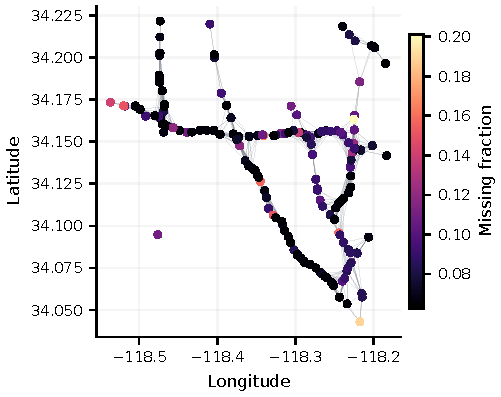
\includegraphics[width=\columnwidth]{figure/traffic_network.pdf}
\caption{Los Angeles sensor network. Node colors show the fraction of readings treated as missing.}
\label{fig:sensor-network}
\end{figure}

We train an STGCN-based predictor~\cite{yu2018stgcn} separately for each dataset. It uses 12 past speed measurements to predict the next 12 steps. We evaluate forecasts 15, 30, and 60 minutes ahead. Training uses Adam with a learning rate of $10^{-3}$ and a batch size of 32. We select the checkpoint with the lowest validation MAE. We treat nonfinite and nonpositive speeds as missing. Missing inputs are filled with the sensor's last available speed~\cite{che2018missing}, or its median training speed if no earlier reading is available.

We estimate uncertainty for one target sensor at a time using predicted and observed speeds from its latest 0, 12, 24, or 48 five-minute slots, or its full available data for interval estimation. Other sensors retain their full available data. We repeat each case for every sensor.

For test evaluation, full data combines the tuning data with the latest 48 five-minute slots available from the calibration data before test forecasts begin. Limited-data cases use only the assigned number of these recent slots. Earlier calibration data from the other sensors determines the interval multipliers. We then evaluate all methods on forecasts whose target speed and 12 input measurements at the target sensor are observed.

\subsection{COVID-19 Hospital Admissions}
\label{sec:second-application-setup}

We use daily counts of confirmed COVID-19 hospital admissions reported by HHS through COVIDcast~\cite{reinhart2021covidcast}. The data and geographic graph are distributed with EpiPatch at \url{https://github.com/Alistair-Turcan/EpiPatch}. The selected period covers 978 days from August 23, 2021, to April 26, 2024. We retain the largest connected component, with 49 locations covering the 48 contiguous states and Washington, D.C., and 109 undirected geographic connections of weight one. The selected data contain no missing values, and zero admissions are valid observations.

We evaluate seven-day-ahead forecasts of hospital admissions. The training period provides each state's normalization factor. A forecast difference becomes available for interval estimation once its corresponding admission count is observed. The experiment uses a retrospective data extract with observations treated as available on their recorded dates.

Each state takes a turn as the target with 0, 7, or 14 recent days of data for interval estimation, or its full available data. Other states retain their full available data. For test evaluation, full data contains 92 days from the tuning period and the latest 14 available days from the calibration period. The earlier 78 calibration days from the other states determine the interval multipliers. We evaluate 92 daily forecasts per state from January 26 to April 26, 2024.

\subsection{Evaluation Metrics}

We compare the three methods at a 90\% coverage target using Winkler score, coverage, and interval width. Winkler score penalizes wide intervals and observations outside them, with lower scores indicating better results~\cite{winkler1972interval,bracher2021evaluating}. Coverage is the fraction of observations inside the intervals. For traffic, both Winkler score and interval width are reported in mph. For hospital admissions, we divide each state's Winkler score by its training-period standard deviation $\tau_j$ to give states with different admission levels comparable influence, while interval width is reported in admissions. Within each application, we average each metric within each location and then equally across locations, separately for each forecast horizon and amount of available data.

Code and instructions for reproducing the experiments are available at \url{https://github.com/Arashlf/graph-smoothed-intervals-mldb}.

\section{Results and Discussion}
\label{sec:evaluation}

We examine how the three approaches compare as the amount of available data changes.

\subsection{Traffic Forecasting Results}

Table~\ref{tab:interval-results} compares scores, coverage, and widths for forecasts 30 minutes ahead using the target sensor's latest 24 five-minute slots. Fig.~\ref{fig:winkler-results} shows the broader comparison in Los Angeles. When we use data from the target sensor's latest 12, 24, or 48 five-minute slots, Graph Smoothing lowers mean Winkler score by 3.3--6.6\% relative to Global and 14.9--22.1\% relative to Local. These ranges cover the three amounts of available data and all forecast horizons. When we use no data from the target sensor to estimate its interval, Graph Smoothing lowers the score by 3.5--7.0\% relative to Global.

\begin{table}[ht]
\caption{Test results for forecasts 30 minutes ahead using the target sensor's latest 24 five-minute slots. Values are sensor averages, with a 90\% coverage target. Bold marks the lowest mean Winkler score in each dataset.}
\label{tab:interval-results}
\centering
\footnotesize
\setlength{\tabcolsep}{5pt}
\begin{tabular}{lrrr}
\hline
Method & Winkler score & Coverage & Width \\
 & (mph) & (\%) & (mph) \\
\hline
\multicolumn{4}{l}{\textit{Los Angeles}} \\
Global & 36.19 & 90.14 & 16.50 \\
Local & 43.93 & 80.53 & 15.94 \\
Graph Smoothing & \textbf{34.66} & 89.82 & 15.88 \\
\hline
\multicolumn{4}{l}{\textit{Bay Area}} \\
Global & 21.64 & 88.27 & 7.06 \\
Local & 23.59 & 78.64 & 6.42 \\
Graph Smoothing & \textbf{21.51} & 87.17 & 6.77 \\
\hline
\end{tabular}
\end{table}

\begin{figure*}[t]
\centering
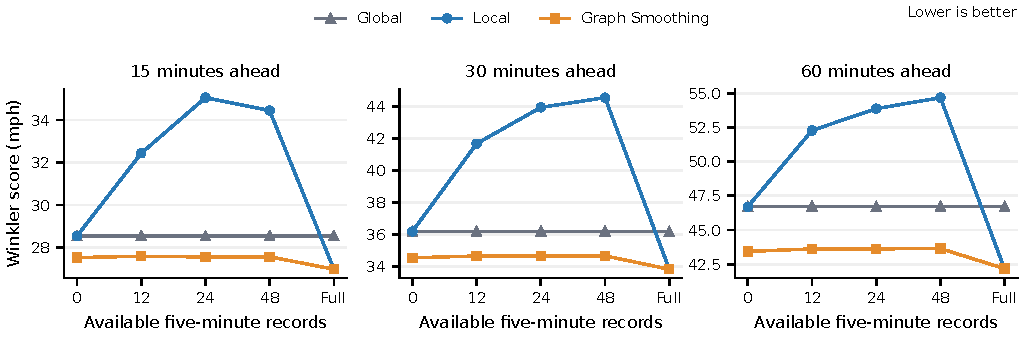
\includegraphics[width=\textwidth]{figure/traffic_winkler_by_history.pdf}
\caption{Mean Winkler score in Los Angeles. We vary the amount of data used to estimate the target sensor's interval. Other sensors retain their full available data. Full uses all data available for interval estimation. Local and Graph Smoothing have nearly identical mean scores at Full.}
\label{fig:winkler-results}
\end{figure*}

In Bay Area, Graph Smoothing lowers mean Winkler score by 6.7--16.4\% relative to Local when we use data from the target sensor's latest 12, 24, or 48 five-minute slots. Its scores are close to Global, differing by less than 1.3\%. When we use no data from the target sensor to estimate its interval, Graph Smoothing gives the same intervals as Local.

Fig.~\ref{fig:sensor-improvements} shows how the score differences vary across Los Angeles sensors. In the cases using 0, 12, 24, or 48 five-minute slots for the target sensor, Graph Smoothing gives lower scores than Global for about 75--80\% of sensors. In Bay Area, it gives lower scores for about 50--58\% of sensors in the cases using 12, 24, or 48 slots, and the median reductions remain near zero. These results show that the average score reductions are shared by more sensors in Los Angeles than in Bay Area.

\begin{figure}[ht]
\centering
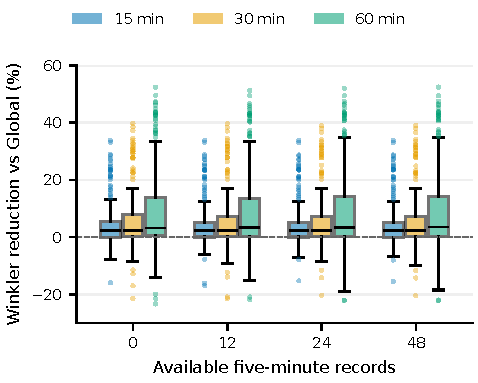
\includegraphics[width=\columnwidth]{figure/traffic_sensor_improvement_vs_global.pdf}
\caption{Sensor-level percentage reductions in Winkler score relative to Global in Los Angeles. Positive values favor Graph Smoothing. Boxes show the middle 50\% of sensors, with a line at the median.}
\label{fig:sensor-improvements}
\end{figure}

When we use the target sensor's full available data, Graph Smoothing gives the same intervals as Local for all three Bay Area forecast horizons and for 15- and 30-minute Los Angeles forecasts. For 60-minute Los Angeles forecasts, their mean Winkler scores differ by about 0.1\%, with Local slightly lower. Local has higher mean Winkler scores when it uses the target sensor's latest 12, 24, or 48 slots than when it uses no data from that sensor. In the latter case, Local calculates the starting scale from the other sensors.

We also examine coverage alongside Winkler score. When we use the target sensor's latest 12, 24, or 48 five-minute slots, Graph Smoothing reaches mean coverage of 89.7--89.9\% in Los Angeles and 86.7--87.5\% in Bay Area, against the 90\% target.

Fig.~\ref{fig:interval-example} shows the intervals for one Los Angeles sensor. Local produces a narrow interval that misses many observed speeds, while Global produces a much wider interval. The Graph Smoothing interval is wider than Local and narrower than Global. We selected this sensor as an example, while the results above summarize all sensors.

\begin{figure}[ht]
\centering
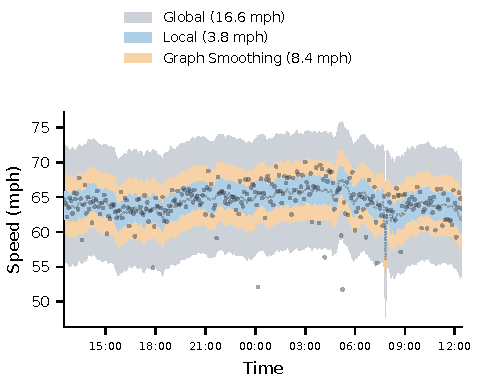
\includegraphics[width=\columnwidth]{figure/traffic_prediction_interval_example.pdf}
\caption{Intervals for a Los Angeles sensor using data from its latest 12 five-minute slots and forecasts 30 minutes ahead. The example sensor is selected using test scores to illustrate a case where Graph Smoothing improves on both alternatives. Bands show prediction intervals, and dots show observed speeds.}
\label{fig:interval-example}
\end{figure}

\subsection{COVID-19 Hospital Admissions Results}
\label{sec:second-application-results}

Graph Smoothing also lowers mean scaled Winkler scores in the hospital-admissions application. Fig.~\ref{fig:hospital-results} compares the three approaches as the target state's available data changes. With 0, 7, and 14 days of target data, Graph Smoothing reduces mean scaled Winkler score by 10.2\%, 5.6\%, and 3.1\% relative to Global, respectively. It also gives lower mean scores than Local in each of these cases. With full available data, Graph Smoothing and Local give the same intervals.

\begin{figure}[ht]
\centering
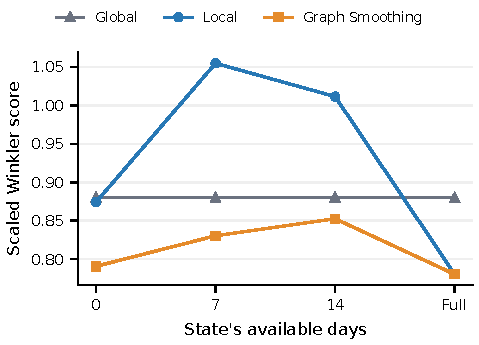
\includegraphics[width=\columnwidth]{figure/hospital_interval_results.pdf}
\caption{Mean scaled Winkler score for seven-day-ahead hospital-admission forecasts. Each state's score is divided by its training-period standard deviation, then scores are averaged equally across locations. Local and Graph Smoothing overlap at Full.}
\label{fig:hospital-results}
\end{figure}

With limited target data, Graph Smoothing gives mean interval widths of 60.5--64.0 admissions, compared with 74.5 for Global. Its mean coverage is 96.7--98.7\%, above the 90\% target. The intervals are narrower than Global's while remaining conservative on average. This application demonstrates the use of the same scale-sharing method around hospital-admission forecasts.

\subsection{Discussion and Limitations}

The benefit of graph smoothing depends on the application and the data available at the target location. Its mean score reductions relative to Global are clearer in Los Angeles and hospital admissions, while its mean scores in Bay Area remain close to Global. With full available data, Graph Smoothing and Local have equal or nearly equal mean scores in all three datasets. The clearest gains from sharing scale information occur when the target location has limited data.

The evaluation uses one test period per dataset, and earlier traffic results from these periods informed the experimental design. Evaluation on additional, unused periods would help assess how well the findings carry over. Our comparisons evaluate the complete method. Comparisons with count-only weights and graph-free shrinkage would help identify how much the variance weights and graph connections each contribute.

\section{Conclusion}
\label{sec:conclusion}

Point forecasts provide an estimated value, while prediction intervals describe a range of plausible observations. Including these intervals helps express uncertainty in forecasts of traffic speeds and hospital admissions. We presented a variance-weighted graph-smoothing method that uses information from connected locations to estimate intervals when a target location has limited data. Our evaluations show how this information sharing can improve prediction intervals in both applications.

Future research could explore privacy-preserving information sharing for interval estimation and updating prediction intervals as traffic or epidemic conditions change. Another direction is to develop a rule for identifying when graph smoothing is useful, based on the amount of available data and differences between connected locations. These directions could make prediction intervals more useful across applications with changing conditions and uneven data availability.

\section*{Acknowledgment}

This work has been supported by the USDA National Institute of Food and Agriculture, grant number 2022-67015-38059 through the NSF/NIH/USDA/BBSRC/BSF/NSFC Ecology and Evolution of Infectious Diseases Program.

\bibliographystyle{IEEEtran}
\bibliography{references}

\end{document}
